\chapter{Backbone}\label{chap:backbone}
The main controller of the application is the backbone. It is constructed by the API at launch, and after its construction it starts its own thread and takes control of the network library.

\section{The backbone class}
The backbone class and its buffers functions like a state machine, it controls the overall flow of the system by repeatedly checking the state of all buffers and deciding which buffer needs attention. The backbone will under all circumstances, as long as there is data in any buffer, dispatch work to one of the layers, so the system is only idle when there is no data left to process.
If more than two buffers have accumulated a sufficient amount of data, it is up to the backbone to choose the most urgent of the two buffers to work with. As this library has ample opportunity to choke itself with data, if it is not properly handled.

The end user application, does not decide how the backbone is allocated explicitly, instead it will be created upon loading the library and instantiating by the API layer. This means that the startup of the library implicitly will be part of the facade pattern.
The backbone class is also responsible for creation of the buffers and for handling settings and errors. 
The sizes of the buffers can ideally be defined through the API layer at runtime, in order to allow a user to adjust the memory footprint of the library. 
However the library should contain good default values, so the user does not need to configure this manually under most circumstances.

The backbone runs in a separate thread to prevent taking execution time from other processes in the user application. This introduces thread racing conditions  (See \ref{thread_race_conditions}) at the API layer, when the user application wishes to send and retrieve a message, data may be lost. Therefore the buffer must be constructed with a way to handle this situation, as this is outside the scope of the backbone itself.

\subsection{Threshold values}
Each of the buffers have an associated minimum and maximum value. Together with their size and data count, they define the response of the backbone when there are borderline congestion.
The minimum value of a buffer is meant as a count of units that the system should aim to have in that buffer when possible. For instance the physical layer buffer needs to have above a certain amount of frames ready to send to its audio layer, because the library cannot guarantee when it can expect to execute next. Therefore the more data there is in the output buffers, the longer the network thread can wait before executing again. This is important, because the library will in the end not be running on a real time system, so execution time is not guaranteed.
The maximum value indicates how much data there can be in a buffer before the system is close to congestion. Therefore whenever there is too much data in a buffer, the backbone should prioritize moving it out.


Too much outgoing data, or too little ingoing data in the system buffers, does not represent a stability threat, and the library will continue to operate at full, or close to full capacity under these circumstances. This means that the minimum threshold values doesn't apply to ingoing buffers, and maximum threshold values doesn't apply to outgoing buffers.


\subsection{Execution flow}
The method for determining which buffer to work with, is based on the following criteria:

In the case of sending messages, the physical layer buffer should never be empty unless all the other buffers are empty, otherwise the library will waste token time. This means that it is of high priority to move frames from the data link layer to the physical layer.
At the same time, there must never be to many frames in the physical input buffer, otherwise data will be lost. Because buffer problems with the physical layer will directly result in erroneous operation of the library, these buffers must have the highest priority, when deciding where to ''work''. The inbound buffers has the highest priority, since faults here cause data loss, where as the other merely causes delays.

Next are the frame buffers. By the same logic these can create congestion when there are to many frames to decode, which will later stall the physical layer. These will have high priority, but lower than the physical layer buffer.
And again the outgoing packet buffers will create a lack of frames if they don't deliver decoded packages.

The same argument goes for the transport layer, which of course has the lowest priority value.
 In the end the final priority queue is:

\begin{enumerate}
\item If amount of input frames \textgreater\, input frame maximum value, move frames from the physical layer.
\item If amount of output frames \textless\, output frames minimum value, move frames to the physical layer.
\item If amount of frames \textgreater\, frame maximum value, decode frames (produces inbound packages).
\item If amount of frames \textless\, frame minimum value, encode packets (produces outbound frames).
\item If amount of packets \textgreater\, package maximum value, decode packets (produces finished inbound messages).
\item If amount of packets \textless\, package minimum value, encode messages (produces outbound packages).
\end{enumerate}


This prioritized flow (see figure \ref{fig:backboneprime}) will ideally ensure that the system strives to stay in a ''stable'' state, during medium load time. 


Even if the library doesn't receive much processing time from the operating system, it should still manage to behave in a manner consistent with the protocol.


When the system is a bit more relaxed, that is, all values are within working parameters, the system will assign work in a way that functions like round robin, which means that the system checks all buffers once, and then if there is no work to be done, goes to sleep for a predetermined amount of time. The first buffer to check is advanced through the six buffers for each attempt at general work, in accordance with flow \ref{fig:backbonegeneral}.




\textbf{An important note:}
Whenever a buffer indicates that it needs to be emptied, it is not enough to just blindly empty the buffer. It is also necessary to check whether the output buffer can hold the result. If it can: great, if it cannot then the buffer that is blocking the action needs to be emptied.
The reason for this is that when a buffer indicates that it needs more items, if the buffer it fetches from is empty, then that buffer needs to be filled first.


Since there isn't a one-to-one correspondence between frames and packages or packages and messages, a buffer checker function needs to be created; One for determining whether there is room for a message to be decoded and one to determine whether the data link layer can execute. The reason that the data link layers decode-and encode-functions aren't viewed independently is that the decode and encode functions always need to be called right after one another. This effectively wraps up into a single data link action, except when the layer indicates otherwise by the needs attention function.
Note that these checks depend on, among other parameters, the maximum size of packages and frames.





\section{The buffer class}
\label{bufferclass}
The buffer class itself is the container of all messages, packets and frames within the library. There are three sets of sub buffers within it: Two message buffers, two package buffers and two frame buffers. 
The message is a bit different from the package buffers and frame buffers, and will be described independently. 

They are used by the backbone to store messages, but the API and by extension the user thread can also pull or push messages from and to them. This introduces a concurrency problem and the message buffer needs to be able to handle the situation of simultaneous access flawlessly.
Since the buffer is used as FIFO storage, it would make sense to be able to put a mutex (see \ref{mutex}) on only the last element of the queue, and implement it as a linked list.
This would allow concurrent access that would not corrupt the list in any way since insertion in no way affects extraction, unless there is only one element in the queue, and here the mutex would guard it.
When compared to the circular buffer offered by boost, or the simple array, there is a significant performance boost to the queue with a locked last element, since the flat array and circular buffer both would need a shared mutex to read and write, and both have a fixed size in order to be effective.
An additional positive thing about the linked list, is that it can grow and shrink at will when needed. The downside is that the space is allocated in the dynamic memory, and therefore possibly represent a point of memory leakage if not designed properly, and it takes up quite a bit of memory compared to the other two alternatives.

The frame buffer and package buffer have different needs compared to the message buffer. There is no need for handling concurrent access, and no explicit need to allocate more storage at runtime, as this will increase the running time of the individual layers.
Therefore a type of circular buffer with fixed size is used instead, ideally with data allocated at startup. So the individual layers doesn't construct any objects at runtime, but instead uses those already allocated by the buffer.
When a layer is used to decode or encode, the only parameters it receives are pointers to the buffers, as that is all the data they need.

\begin{figure}[htb]
	\begin{center}
	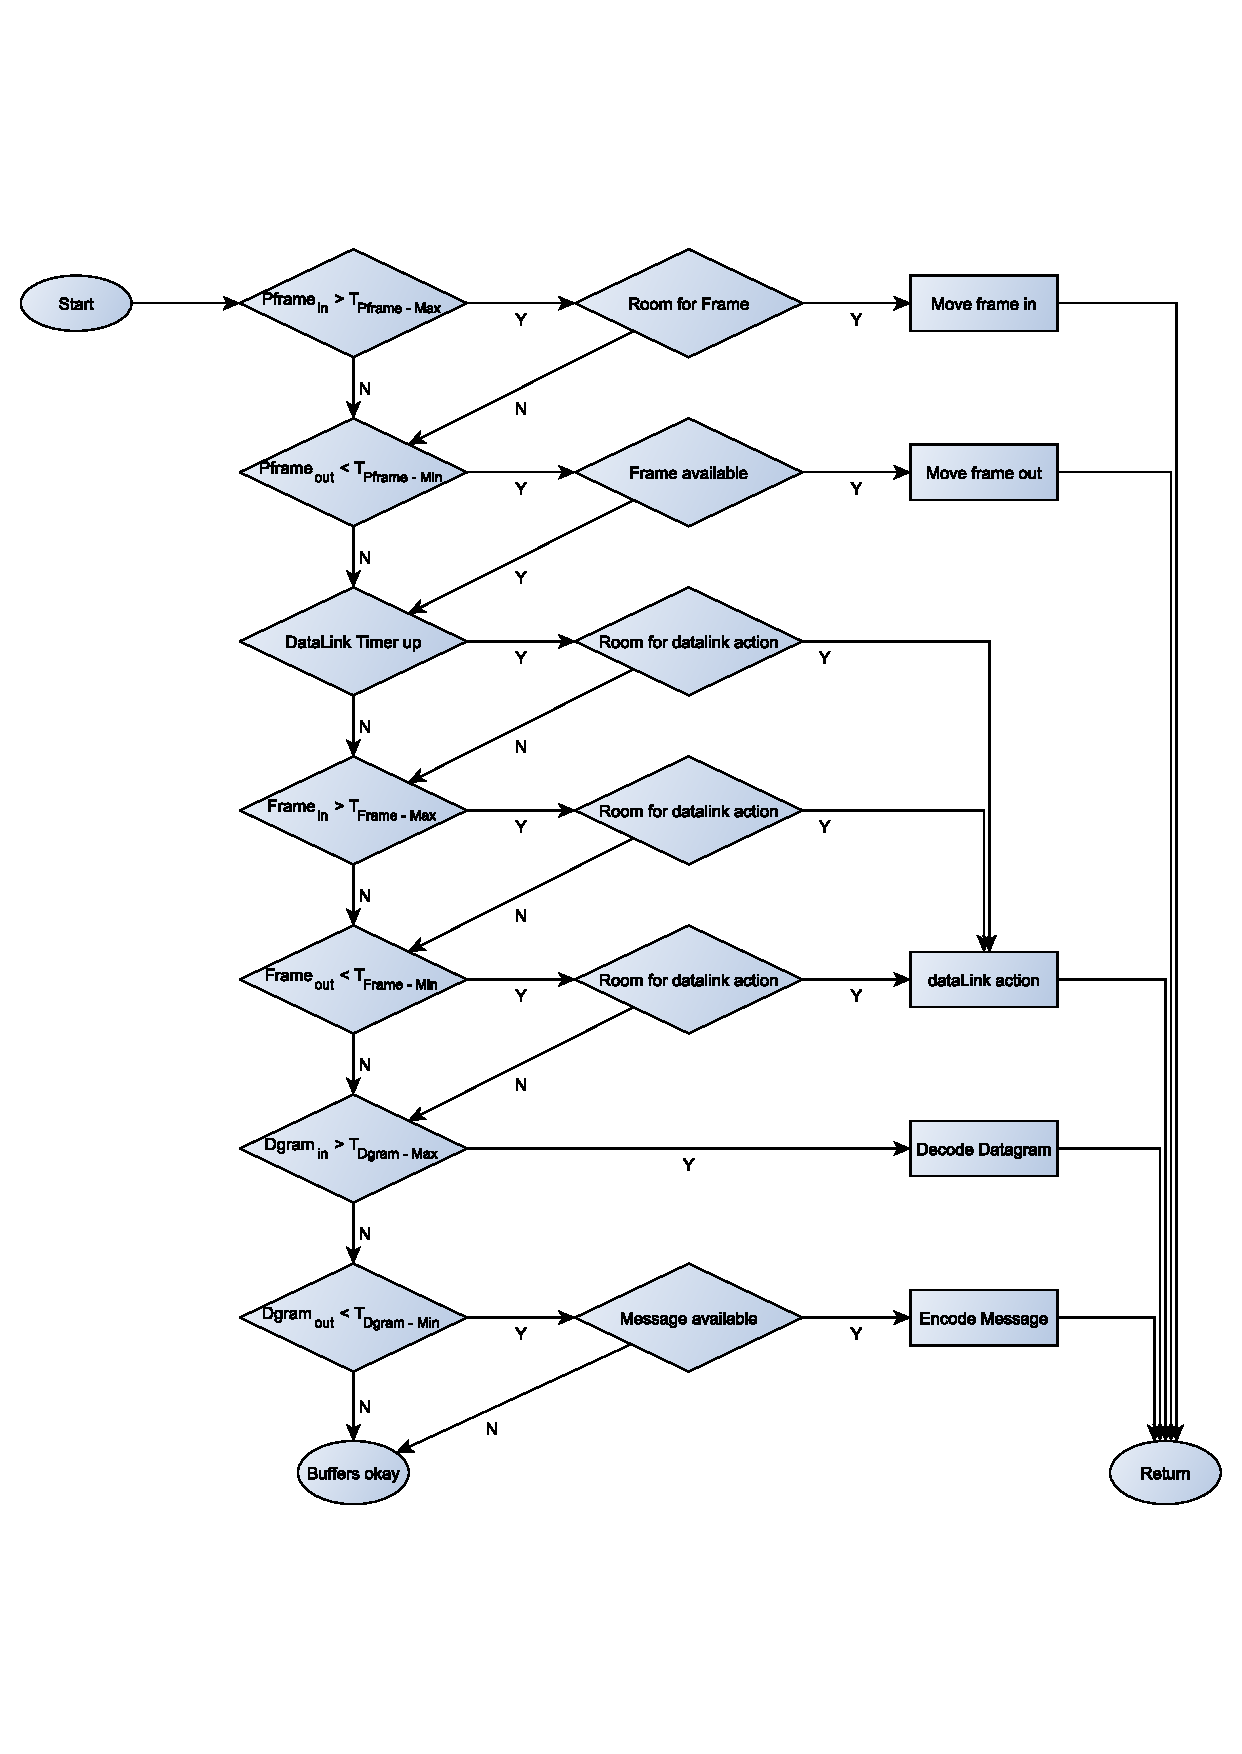
\includegraphics[scale=0.66,trim=0 100 0 100]{backbonePrime.pdf}
	\caption{Backbone primary flow. This diagram illustrates the decision process when determining what buffers to service. ''P. frames'' are frames still buffered in the physical layer.}
	\label{fig:backboneprime}	
	\end{center}
\end{figure}

\begin{figure}[htb]
	\begin{center}
	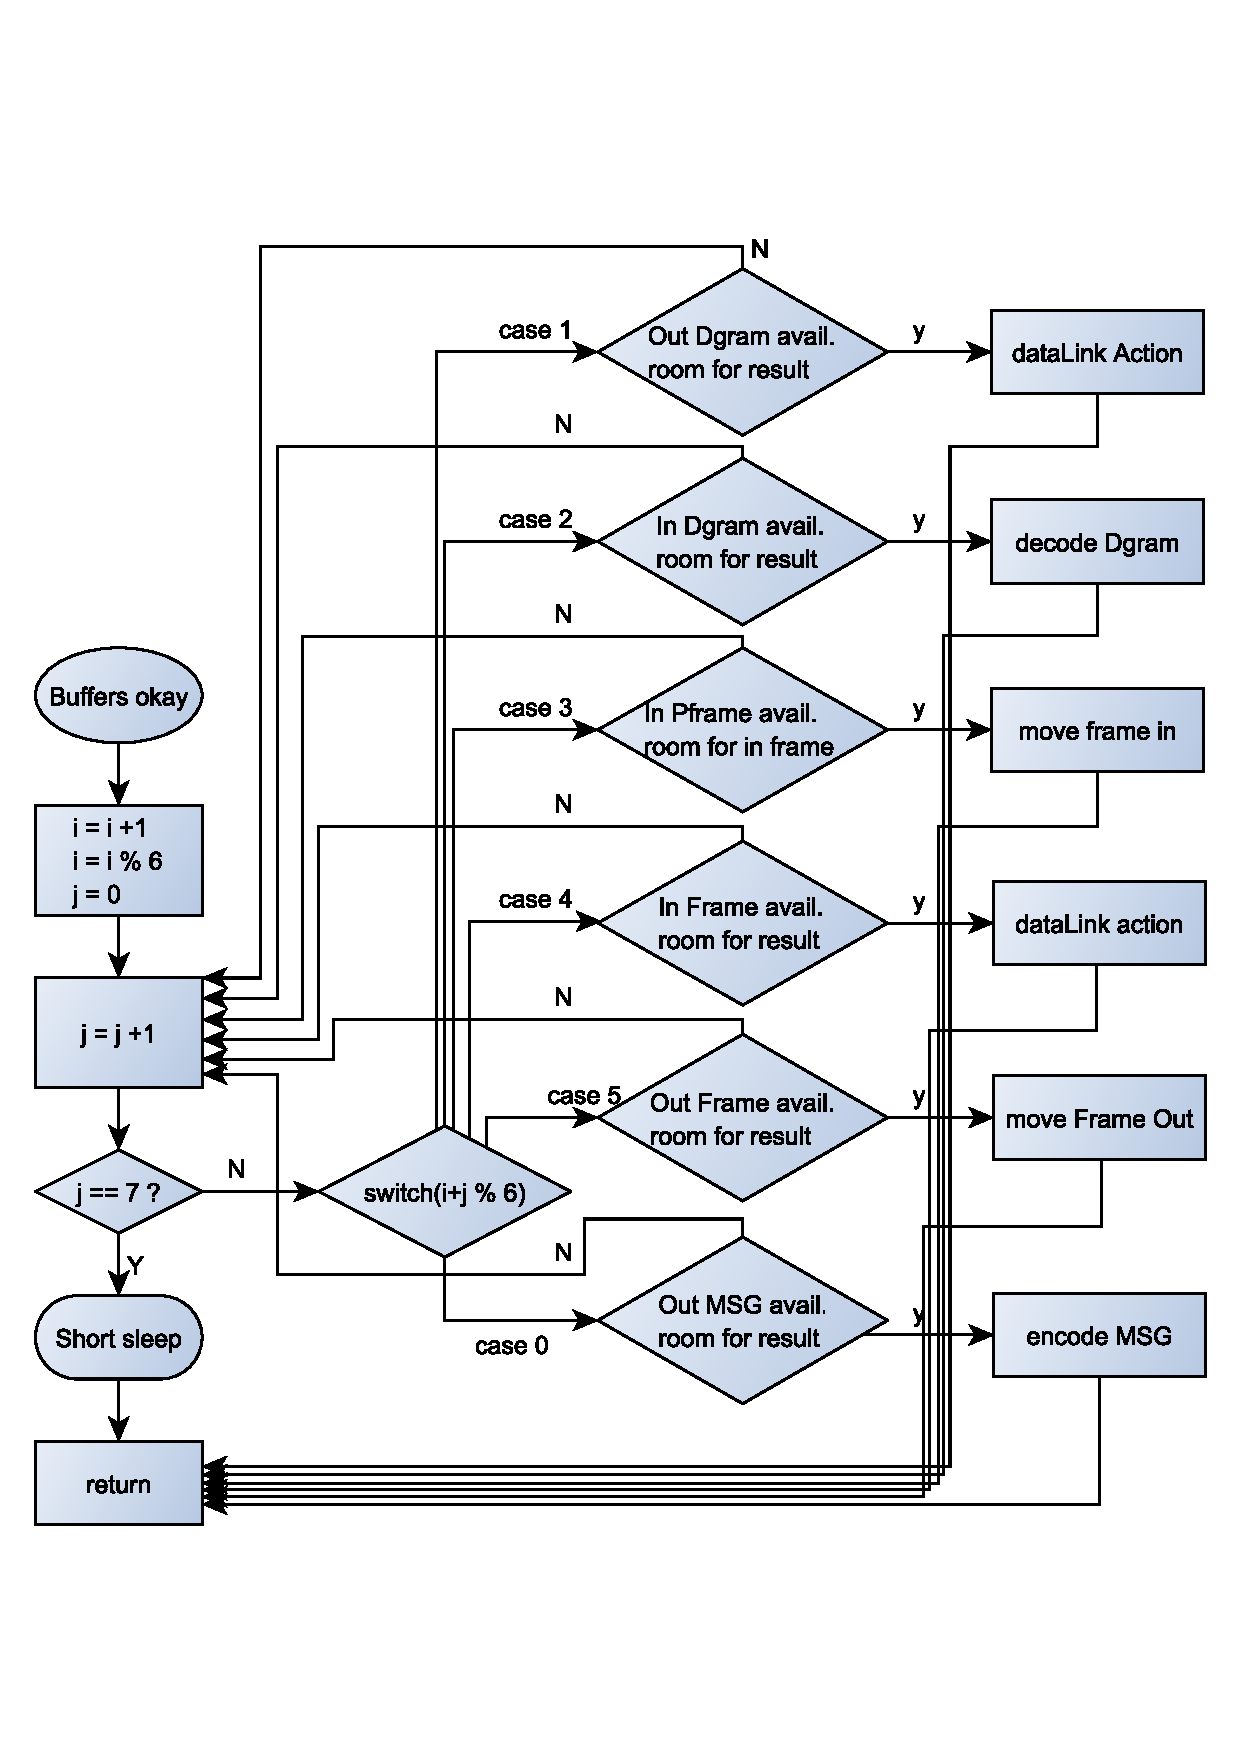
\includegraphics[scale=0.66,trim=0 100 0 100]{backboneGeneral.pdf}
	\caption{Backbone general flow. This diagram illustrates the decision process when the system is in a stable state, here the ''switch'' loop, ensures that all 6 actions are evaluated in order, but starting from a different one each time. ''P. frames'' are frames still buffered in the physical layer.}
	\label{fig:backbonegeneral}	
	\end{center}
\end{figure}
